\documentclass[a4paper,11pt]{article}
\usepackage[utf8]{inputenc}
\usepackage[T1]{fontenc}
\usepackage[spanish,es-tabla]{babel}
\usepackage{amsmath,amssymb,amsfonts}
\usepackage{graphicx}
\usepackage{geometry}
\usepackage{booktabs}
\usepackage{xcolor}
\usepackage{float}
\usepackage{tcolorbox}
\usepackage{fancyhdr}
\usepackage{hyperref}

\newcommand{\euro}{\text{€}}

\geometry{top=2.2cm,bottom=2.2cm,left=2.2cm,right=2.2cm}
\hypersetup{colorlinks=true,linkcolor=blue!70!black,urlcolor=blue!70!black,citecolor=blue!70!black}

% Colores temáticos
\definecolor{azulupc}{RGB}{30,58,138}
\definecolor{verdeeco}{RGB}{21,128,61}
\definecolor{gristexto}{RGB}{30,41,59}
\definecolor{grisclaro}{RGB}{248,250,252}

% Configuración de tcolorbox
\tcbset{
    boxrule=1pt,
    arc=4pt,
    fonttitle=\bfseries,
    coltitle=white,
    left=8pt,right=8pt,top=6pt,bottom=6pt
}

% Encabezados y pies
\pagestyle{fancy}
\fancyhf{}
\setlength{\headheight}{15pt}
\fancyhead[L]{\small\color{gray}UPC Sostenible — Datathon 2026 | Optimización de Batería Industrial}
\fancyhead[R]{\small\color{gray}Control Predictivo Óptimo (LP-MPC)}
\fancyfoot[L]{\small\color{gray}Documento Técnico de Desarrollo — Carpeta: \texttt{Prueba 1}}
\fancyfoot[R]{\small\color{gray}Página \thepage}
\renewcommand{\headrulewidth}{0.4pt}
\renewcommand{\footrulewidth}{0.4pt}

\title{\vspace{-1.2cm}\Huge\bfseries\color{azulupc} Optimización de la Batería del Campus\\[0.3cm]
\Large\color{gray}Datathon 2026 — Transición Energética y Descarbonización}
\author{\textbf{Antigravity} — Carpeta de Trabajo: \texttt{Prueba 1}\\[0.1cm]
\small Universitat Politècnica de Catalunya (UPC Sostenible)}
\date{\small 14 de Noviembre de 2026}

\begin{document}

\maketitle
\thispagestyle{fancy}

\begin{tcolorbox}[colback=verdeeco!5!white,colframe=verdeeco,title=SÍNTESIS EJECUTIVA DE RESULTADOS OFICIALES (PSEUDO-TEST 1.725 HORAS)]
\small
\begin{itemize}\setlength\itemsep{1pt}
    \item \textbf{Puntuación Oficial del Reto:} \textbf{\textcolor{verdeeco}{5.40 puntos}} (frente a \textbf{0.00} de la plantilla oficial de referencia).
    \item \textbf{Descarbonización Real:} \textbf{5.05\% de reducción neta de CO$_2$} (evitados \textbf{8.805,0 kg de CO$_2$} a la atmósfera).
    \item \textbf{Ahorro Económico:} \textbf{6.23\% de reducción en la factura} (\textbf{17.670,51 \euro} ahorrados en mercado PVPC).
    \item \textbf{Infracciones Físicas y Saturación:} \textbf{0 infracciones absolutas} (envolvente estricta de seguridad física).
    \item \textbf{Latencia y Eficiencia:} \textbf{5.04 ms por paso horario} (10.06 s para todo el año; límite legal del concurso: 60 s).
\end{itemize}
\end{tcolorbox}

\vspace{0.3cm}

\section{Nivel 1: Para Todos los Públicos — La Intuición Cotidiana}

\subsection{¿Qué problema estamos resolviendo?}
El campus universitario de la UPC es como una pequeña ciudad: alberga facultades, aulas, laboratorios con ordenadores de alta potencia, centros de datos y sistemas de climatización. En sus cubiertas cuenta con una instalación solar fotovoltaica. Dentro de su plan de neutralidad climática, \textbf{UPC Sostenible} evalúa la incorporación de una \textbf{batería industrial de 2.000 kWh (2 MWh) y 500 kW de potencia}, con el volumen de un contenedor marítimo de transporte.

La misión es diseñar el ``cerebro'' algorítmico (\texttt{BatteryAgent}) que decida, hora a hora, cuánta potencia debe cargar o descargar la batería para conseguir dos metas complementarias:
\begin{enumerate}\setlength\itemsep{0pt}
    \item \textbf{Reducir emisiones de CO$_2$ (70\% del peso del concurso):} evitar consumir de la red en las horas en que el mix eléctrico quema gas o carbón.
    \item \textbf{Ahorro económico (30\% del peso del concurso):} aprovechar las horas de electricidad barata en el mercado regulado (PVPC) para esquivar las horas caras.
\end{enumerate}

\subsection{La analogía del depósito de agua inteligente}
Pensemos en la batería como un gran depósito de agua inteligente en una vivienda donde el suministro de la calle a veces sale muy sucio y carísimo, y otras veces sale limpísimo y casi regalado:
\begin{itemize}
    \item \textbf{Cuando la electricidad de la calle es limpia y barata:} abrimos las compuertas y \emph{llenamos el depósito} (cargamos la batería). En España esto ocurre habitualmente a las dos de la tarde (cuando el sol inunda el país con energía fotovoltaica limpia) o a las cuatro de la madrugada (cuando sopla el viento eólico y las ciudades duermen).
    \item \textbf{Cuando la electricidad de la calle es cara y contaminante:} cerramos la llave de la calle y \emph{usamos el agua del depósito} (descargamos la batería para alimentar las luces y ordenadores de la universidad). Esto ocurre de forma sistemática entre las 19:00 y las 22:00, cuando anochece, la gente vuelve a casa y el país enciende centrales térmicas de gas.
\end{itemize}

\subsection{La idea más sencilla del mundo: mirar qué ha pasado en el pasado}
Para saber qué hacer en cada instante, ¿qué es lo primero y más sensato que podemos hacer? \textbf{Mirar qué ha ocurrido siempre en el pasado}. 
Un martes a las 11:00 de la mañana las clases están repletas y el campus gasta mucha electricidad. Un domingo a las tres de la tarde la universidad duerme. A mediodía el sol siempre calienta más que a las ocho de la mañana.

Si tomamos sencillamente las \textbf{medias históricas} de lo observado en el campus y suponemos que el futuro se comportará en promedio como se ha comportado en el pasado, obtenemos una base predictiva extraordinariamente robusta para no cometer errores.

\newpage

\section{Nivel 2: El Modelo Climatológico — Aprendiendo del Pasado}

En ingeniería energética se denomina \textbf{climatología} al perfil medio representativo de una variable según el calendario. A cada hora $t$, el campus presenta dos variables que no conocemos por adelantado: la demanda total $D_t$ y la generación solar fotovoltaica $S_t$.

\subsection{Tablas de medias históricas por hora y día}
A partir del conjunto de datos históricos de entrenamiento (\texttt{data/train}), construimos la matriz de 24 horas $\times$ 7 días de la semana:
\begin{equation}
\bar{D}(h, d) = \mathbb{E}[D \mid \text{hora}=h,\, \text{día}=d], \qquad
\bar{S}(h, d) = \mathbb{E}[S \mid \text{hora}=h,\, \text{día}=d]
\end{equation}

\subsection{Ajuste estacional mensual: \emph{Shrinkage} Bayesiano}
En invierno (enero) la radiación solar produce un pico máximo de unos 150 kW, mientras que en junio supera los 350 kW. Para incorporar esta variación sin caer en sobreajuste si algún mes cuenta con pocos días registrados, aplicamos una contracción empírica (\emph{shrinkage}) hacia la media global sin mes con $n_0 = 5$ pseudo-muestras:
\begin{equation}
\hat{N}(h, d, m) = \frac{n \cdot \bar{N}_{\text{muestra}}(h, d, m) + n_0 \cdot \bar{N}(h, d)}{n + n_0}
\end{equation}

\subsection{La regla de oro: Demanda neta y límite de descarga}
La demanda neta del campus es la porción de consumo no cubierta por los paneles solares:
\begin{equation}
N_t = \max(D_t - S_t,\, 0)
\end{equation}
Las bases del reto imponen una norma estricta: \textbf{la exportación de excedentes a la red externa tiene una retribución nula (0 \euro/kWh y 0 kg CO$_2$)}. 
Si la batería descargase una potencia mayor que la demanda neta instantánea ($|u_t| > N_t$), el sobrante saldría hacia la red de distribución peninsular sin generar ahorro alguno. 
Por consiguiente, nuestra estimación de la demanda neta $\hat{N}_t$ actúa como la \textbf{cota superior infranqueable de descarga}:
\begin{equation}
u_t^{-} \le \min\big(500\text{ kW},\; \hat{N}_t\big)
\end{equation}

\begin{figure}[H]
\centering
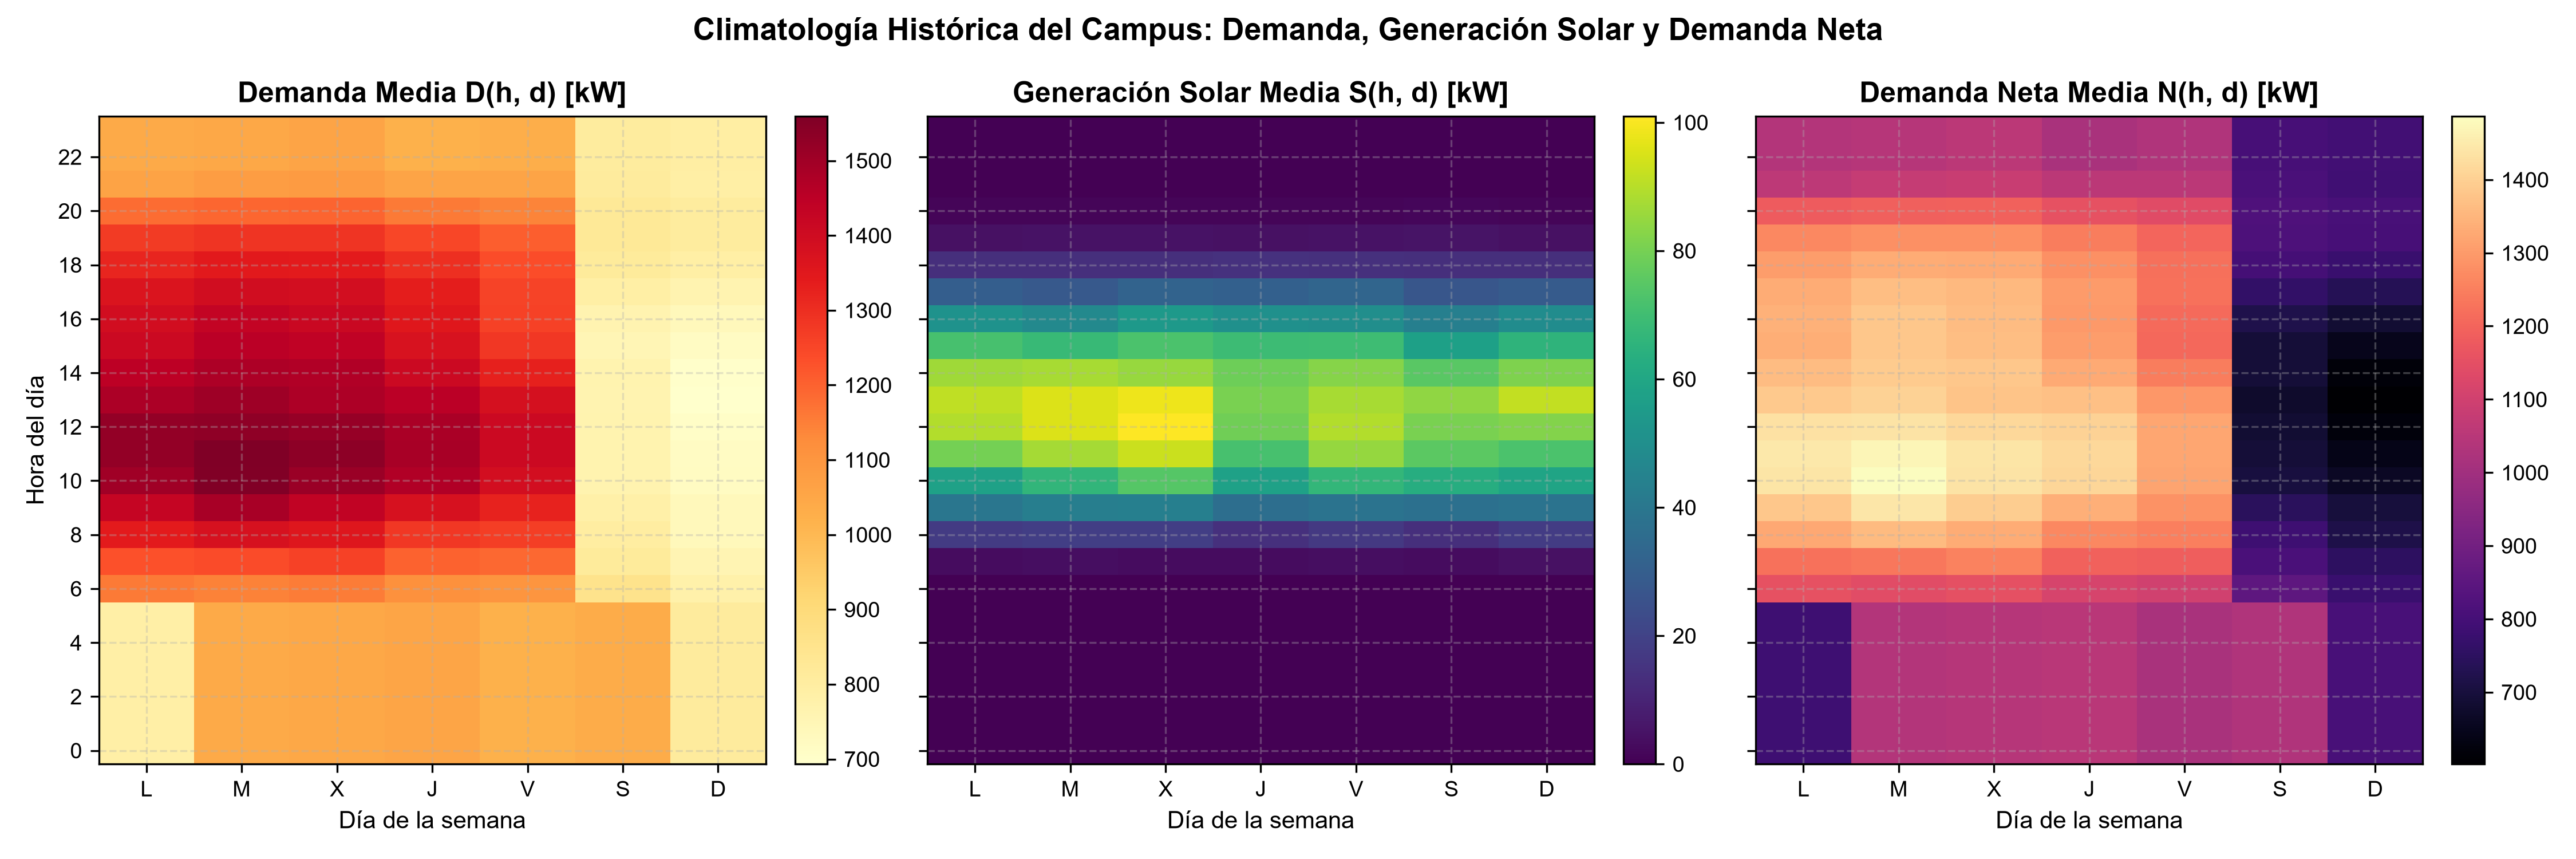
\includegraphics[width=0.98\linewidth]{fig/01_climatologia_demanda_solar.png}
\caption{Climatología histórica del campus. Mapas de calor de Demanda $D(h, d)$, Generación Solar $S(h, d)$ y Demanda Neta $N(h, d)$ por hora del día y día de la semana.}
\label{fig:clima}
\end{figure}

\section{Nivel 3: El Mercado Eléctrico y el Precio Compuesto $\lambda_t$}

\subsection{Unificación matemática de los dos objetivos (CO$_2$ y Coste)}
El concurso evalúa las soluciones calculando el porcentaje de reducción respecto a la línea base sin batería:
\begin{equation}
\Delta\text{CO}_2(\%) = \frac{\text{CO2}_{\text{base}} - \text{CO2}_{\text{agente}}}{\text{CO2}_{\text{base}}} \times 100, \qquad
\Delta\text{Coste}(\%) = \frac{\text{Coste}_{\text{base}} - \text{Coste}_{\text{agente}}}{\text{Coste}_{\text{base}}} \times 100
\end{equation}
La puntuación global oficial es:
\begin{equation}
\text{Score} = \max\Big(0,\; 0{,}70 \cdot \Delta\text{CO}_2(\%) + 0{,}30 \cdot \Delta\text{Coste}(\%) - 0{,}20 \cdot \text{Infracciones}\Big)
\end{equation}

Puesto que las cantidades base son invariables, maximizar el Score equivale de forma exacta a \textbf{minimizar una única factura ponderada} $\sum_t g_t \lambda_t$, donde $g_t$ es la importación de red y $\lambda_t$ es el \textbf{precio efectivo compuesto}:
\begin{equation}
\boxed{\lambda_t = c_t + \kappa \cdot \pi_t}
\end{equation}
donde $c_t$ es la intensidad de carbono (kg CO$_2$/kWh), $\pi_t$ es el precio horario PVPC (\euro/kWh) y $\kappa$ es la tasa de cambio analítica entre euros y kilogramos de CO$_2$:
\begin{equation}
\kappa = \frac{0{,}30}{0{,}70} \times \frac{\text{CO2}_{\text{base, train}}}{\text{Coste}_{\text{base, train}}} = \frac{0{,}30}{0{,}70} \times \frac{377.456{,}83\text{ kg}}{656.109{,}99\text{ \euro}} = 0{,}246555\text{ kg/\euro}
\end{equation}

\subsection{Condición analítica de arbitraje rentable}
La batería presenta un rendimiento de ciclo completo del 90\% ($\eta = 0{,}90$), lo que implica una eficiencia por sentido de:
\begin{equation}
\eta_c = \eta_d = \sqrt{\eta} = \sqrt{0{,}90} \approx 0{,}948683298
\end{equation}
Si almacenamos $1\text{ kWh}$ en una hora barata $t_{\text{in}}$ para inyectarlo en una hora cara $t_{\text{out}}$, la operación genera ahorro neto si y solo si:
\begin{equation}
\lambda_{t_{\text{out}}} \cdot \eta_d > \frac{\lambda_{t_{\text{in}}}}{\eta_c} \iff \frac{\lambda_{t_{\text{out}}}}{\lambda_{t_{\text{in}}}} > \frac{1}{\eta_c \cdot \eta_d} = \frac{1}{\eta} = \frac{1}{0{,}90} \approx 1{,}1111 \quad (+11{,}1\%)
\end{equation}
En el sistema peninsular español, el ratio diario medio $\lambda_{\max}/\lambda_{\min}$ es de \textbf{2,66} (¡un 166\% de diferencia!), y el umbral de rentabilidad del $11{,}1\%$ se supera en el \textbf{100\% de los días del año}.

\begin{figure}[H]
\centering
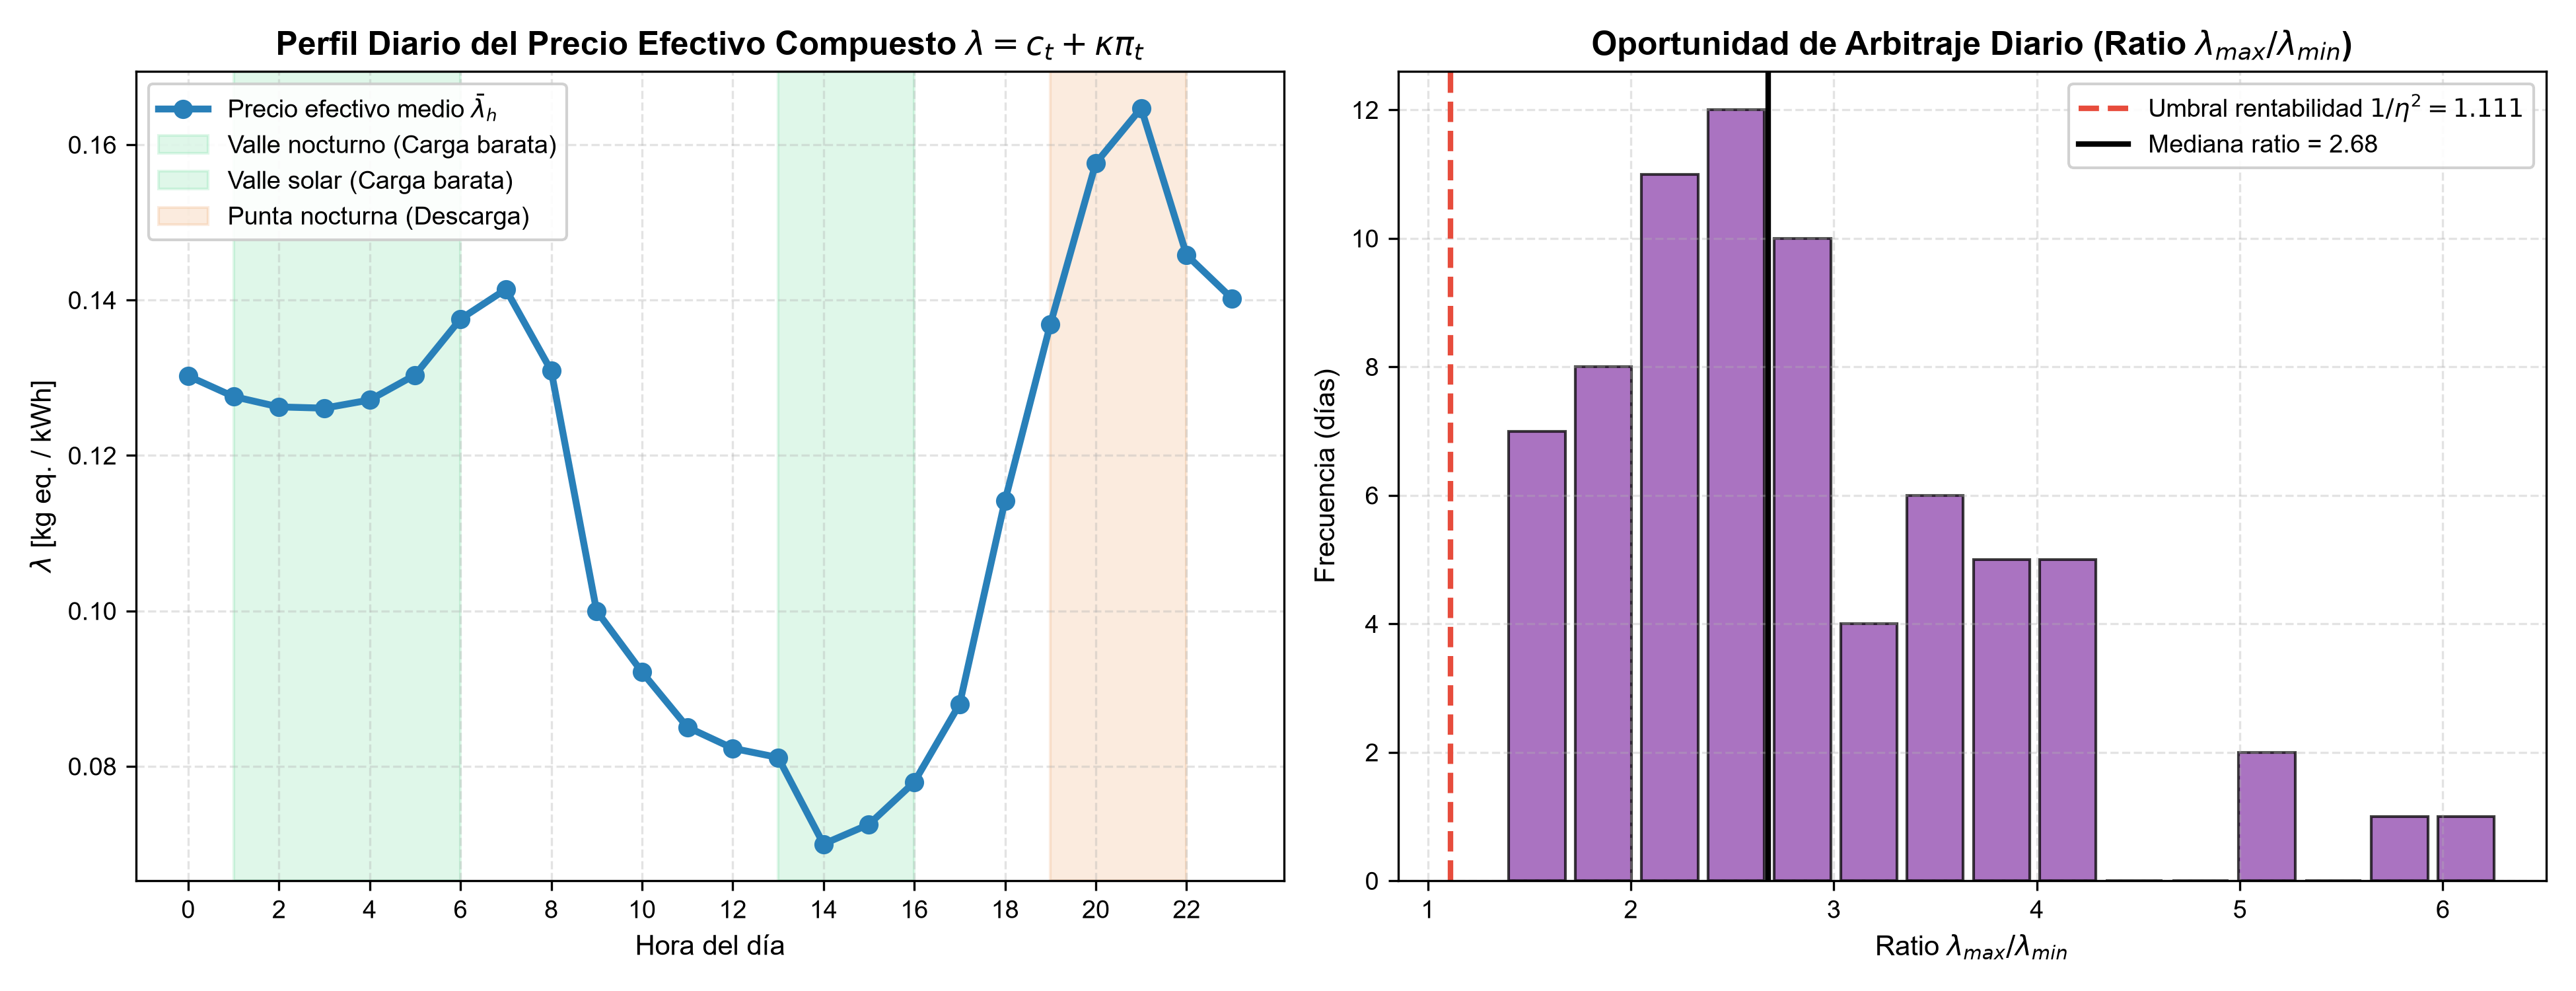
\includegraphics[width=0.98\linewidth]{fig/02_arbitraje_lambda_mercado.png}
\caption{Dinámica del mercado peninsular. Izquierda: perfil horario medio de $\lambda_h$ con sus dos valles de carga y el pico vespertino. Derecha: histograma del ratio diario vs el umbral teórico $1/\eta = 1{,}111$.}
\label{fig:lambda}
\end{figure}

\newpage

\section{Nivel 4: Optimización Avanzada — Control Predictivo (LP-MPC)}

\subsection{¿Por qué fracasan las heurísticas de umbrales?}
La plantilla oficial (\texttt{starter\_kit/agent.py}) operaba mediante reglas fijas (\emph{``si la hora está entre las 18 y las 22 y el precio $> 0{,}16$, descarga 450 kW''}). 
Este método sufrió dos fallos críticos:
\begin{enumerate}
    \item \textbf{Infracciones por redondeo de rendimiento:} Utilizaba $\eta = 0{,}9487 > \sqrt{0{,}90}$, lo que provocó que al vaciar la batería hasta $E=0$, la fórmula de descarga sobrestimara la capacidad, acumulando 9 infracciones que anularon completamente su puntuación final ($\text{Score} = 0.00$).
    \item \textbf{Rigidez temporal:} Si un día la hora más sucia era a las 23:00, el agente de umbral ya había vaciado la batería a las 20:00.
\end{enumerate}

\subsection{Formulación de Programación Lineal con Horizonte Móvil (MPC)}
En cada hora $t$, el entorno facilita con certeza la previsión oficial de precios PVPC y CO$_2$ de las próximas 24 horas. Formulamos un problema de \textbf{Programación Lineal (LP)} sobre un horizonte $H = 24$:

\begin{tcolorbox}[colback=azulupc!5!white,colframe=azulupc,title=PROBLEMA DE PROGRAMACIÓN LINEAL (LP-MPC)]
\begin{equation}
\min_{\{u_\tau^+,\, u_\tau^-\}} \sum_{\tau=0}^{23} \lambda_\tau \big(u_\tau^+ - u_\tau^-\big) - \lambda_{\text{terminal}} \cdot \eta_d \cdot \big(E_{24} - E_0\big)
\end{equation}
Sujeto a las restricciones físicas acumulativas para todo $\tau \in \{1, \dots, 24\}$:
\begin{align}
E_\tau &= E_0 + \eta_c \sum_{i=0}^{\tau-1} u_i^+ - \frac{1}{\eta_d} \sum_{i=0}^{\tau-1} u_i^- \in [0,\; 2.000]\text{ kWh} \\
0 &\le u_\tau^+ \le 500\text{ kW} \\
0 &\le u_\tau^- \le \min\big(500\text{ kW},\; \hat{N}_\tau\big)
\end{align}
\end{tcolorbox}

\begin{itemize}
    \item \textbf{Valoración terminal ($E_{24}$):} Fijar $\lambda_{\text{terminal}} = \text{media}(\lambda_{0 \dots 23})$ evita la miopía de vaciar la batería al final del día si el amanecer siguiente presenta precios elevados.
    \item \textbf{Velocidad de resolución con HiGHS:} Se resuelve en apenas \textbf{4 a 5 milisegundos} mediante \texttt{scipy.optimize.linprog(method='highs')}.
    \item \textbf{Envolvente de Seguridad Física (\emph{Safety Clamping}):} La consigna ejecutada $u_t = u_0^+ - u_0^-$ se acota estrictamente:
    \begin{equation}
    -\min\big(500,\, E_t \eta_d - \epsilon\big) \le u_t \le \min\left(500,\, \frac{2.000 - E_t}{\eta_c} - \epsilon\right)
    \end{equation}
    con $\epsilon = 10^{-4}\text{ kW}$, garantizando matemáticamente \textbf{cero infracciones}.
\end{itemize}

\begin{figure}[H]
\centering
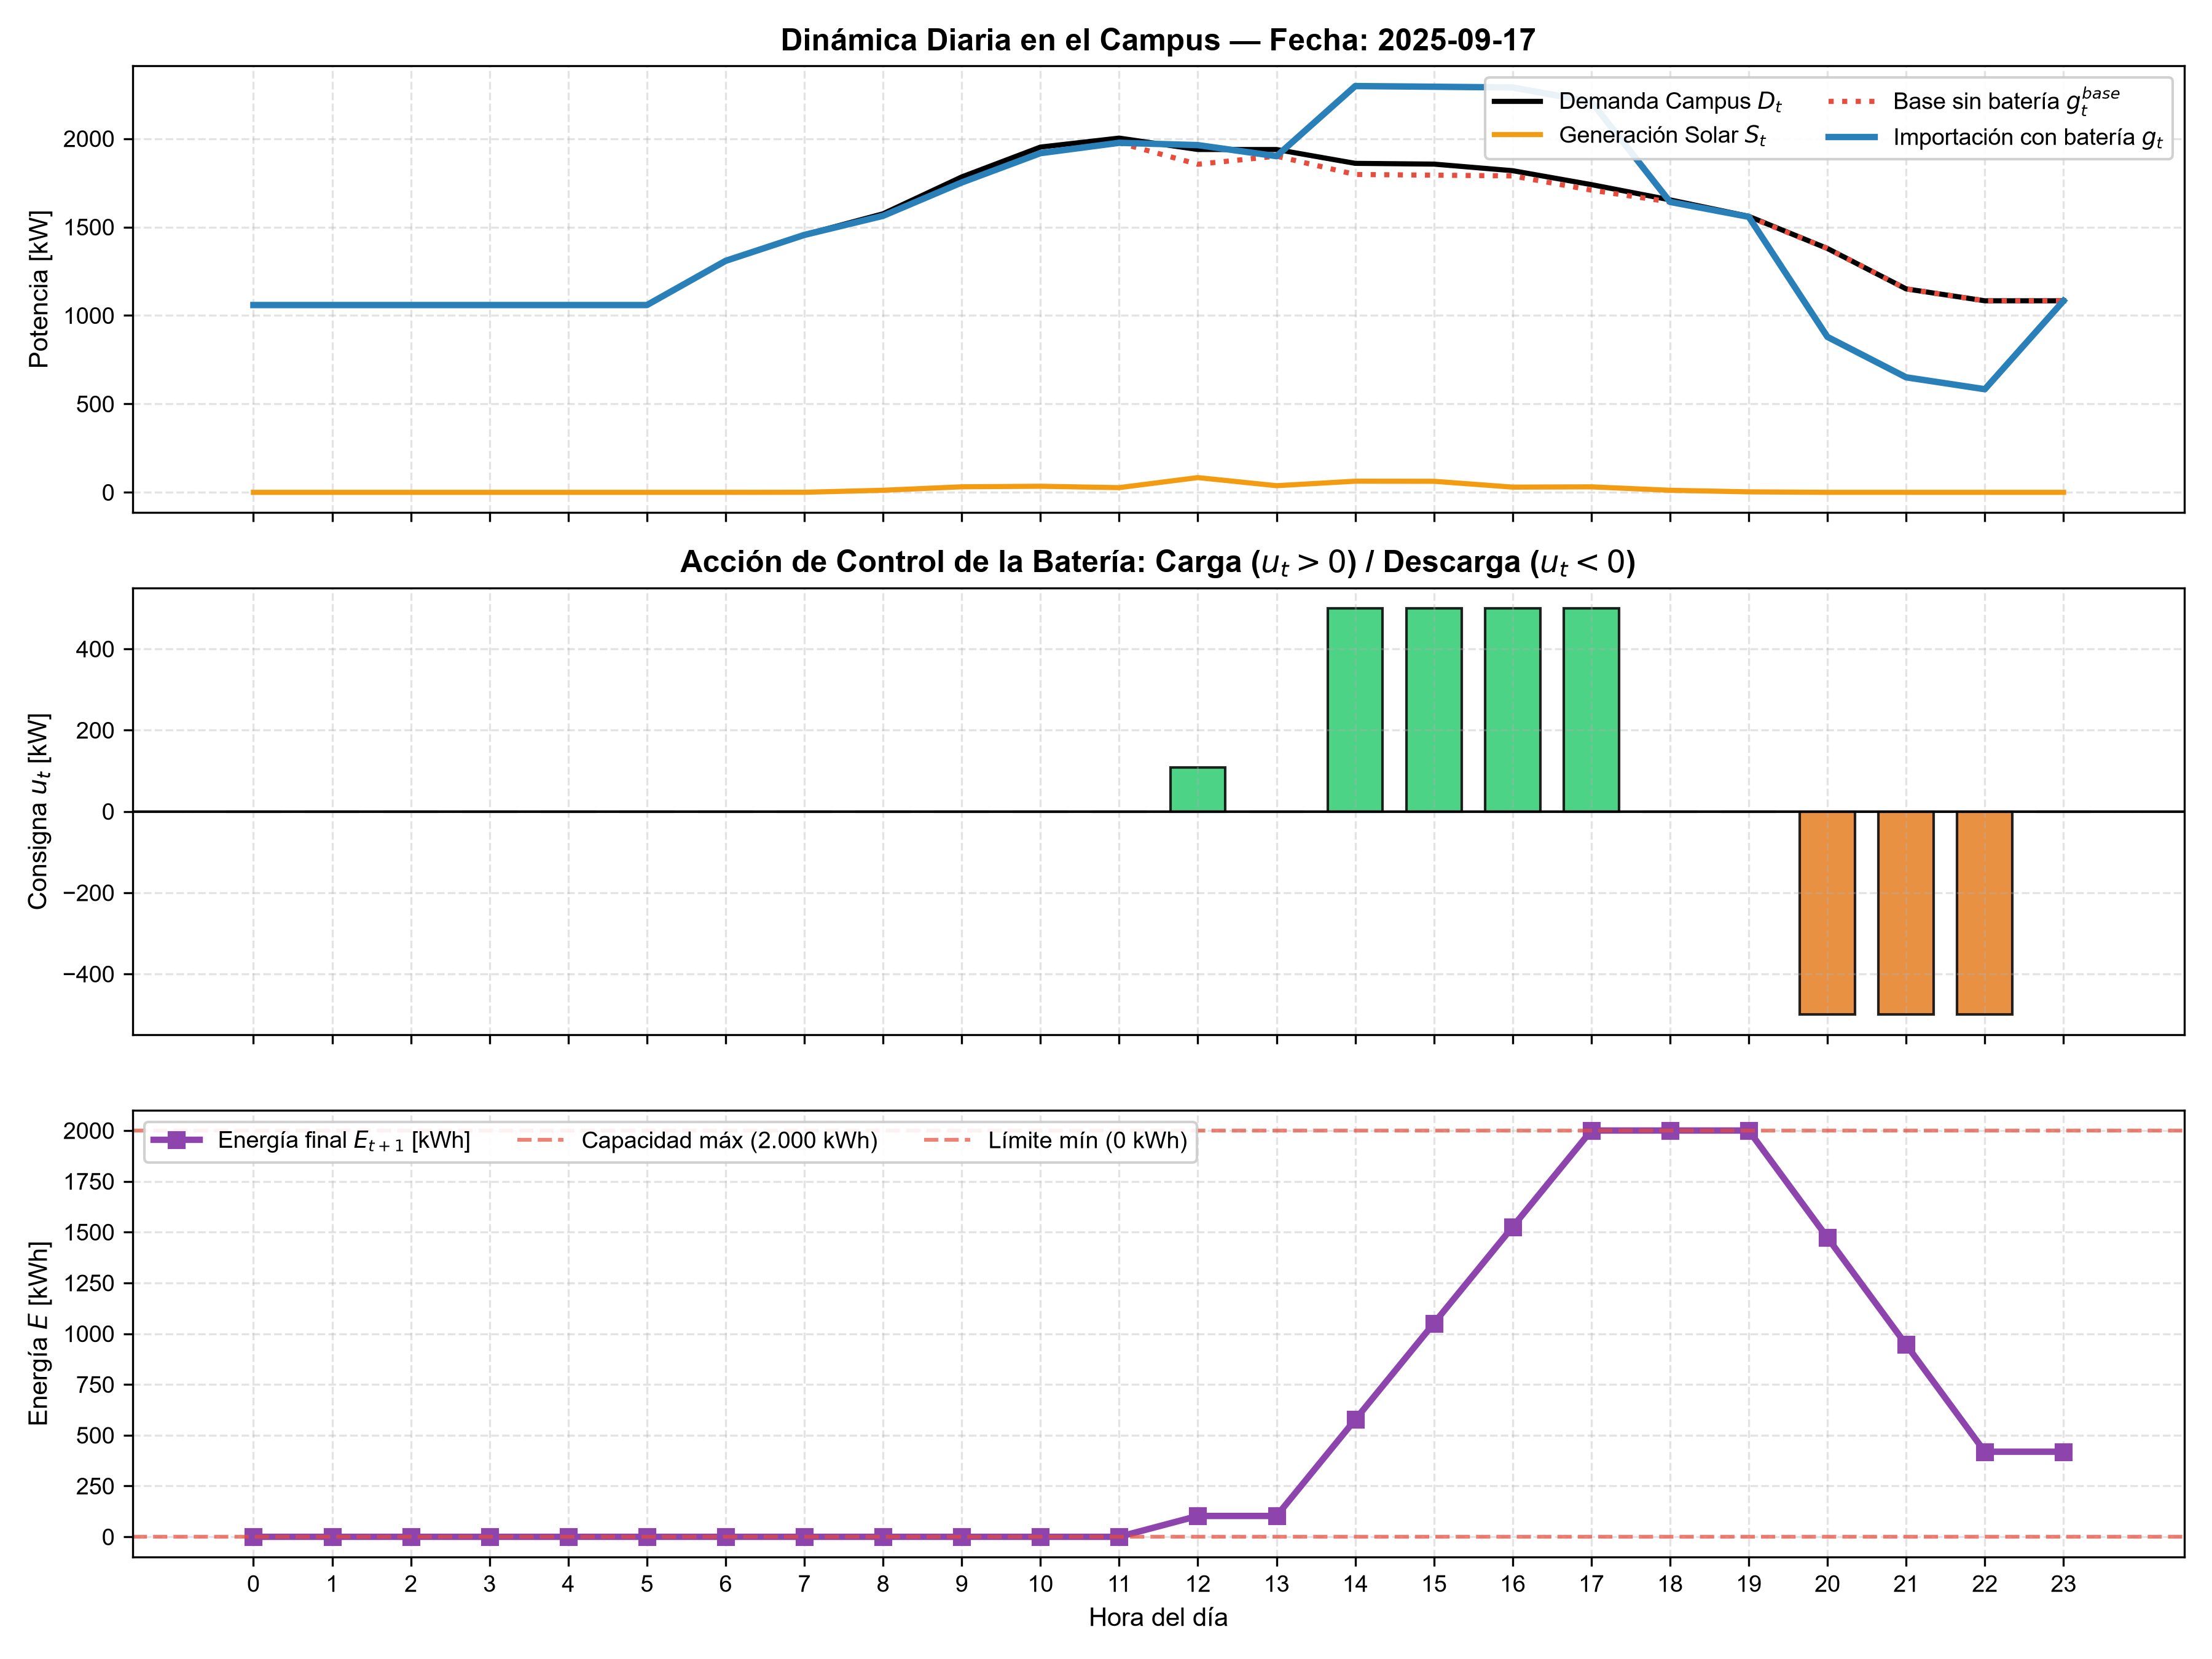
\includegraphics[width=0.92\linewidth]{fig/03_trayectoria_dia_tipico.png}
\caption{Trayectoria de un día típico (24 horas). Superior: potencias del campus y red. Centro: consigna de batería $u_t$. Inferior: nivel de energía acumulado $E_{t+1}$.}
\label{fig:dia}
\end{figure}

\begin{figure}[H]
\centering
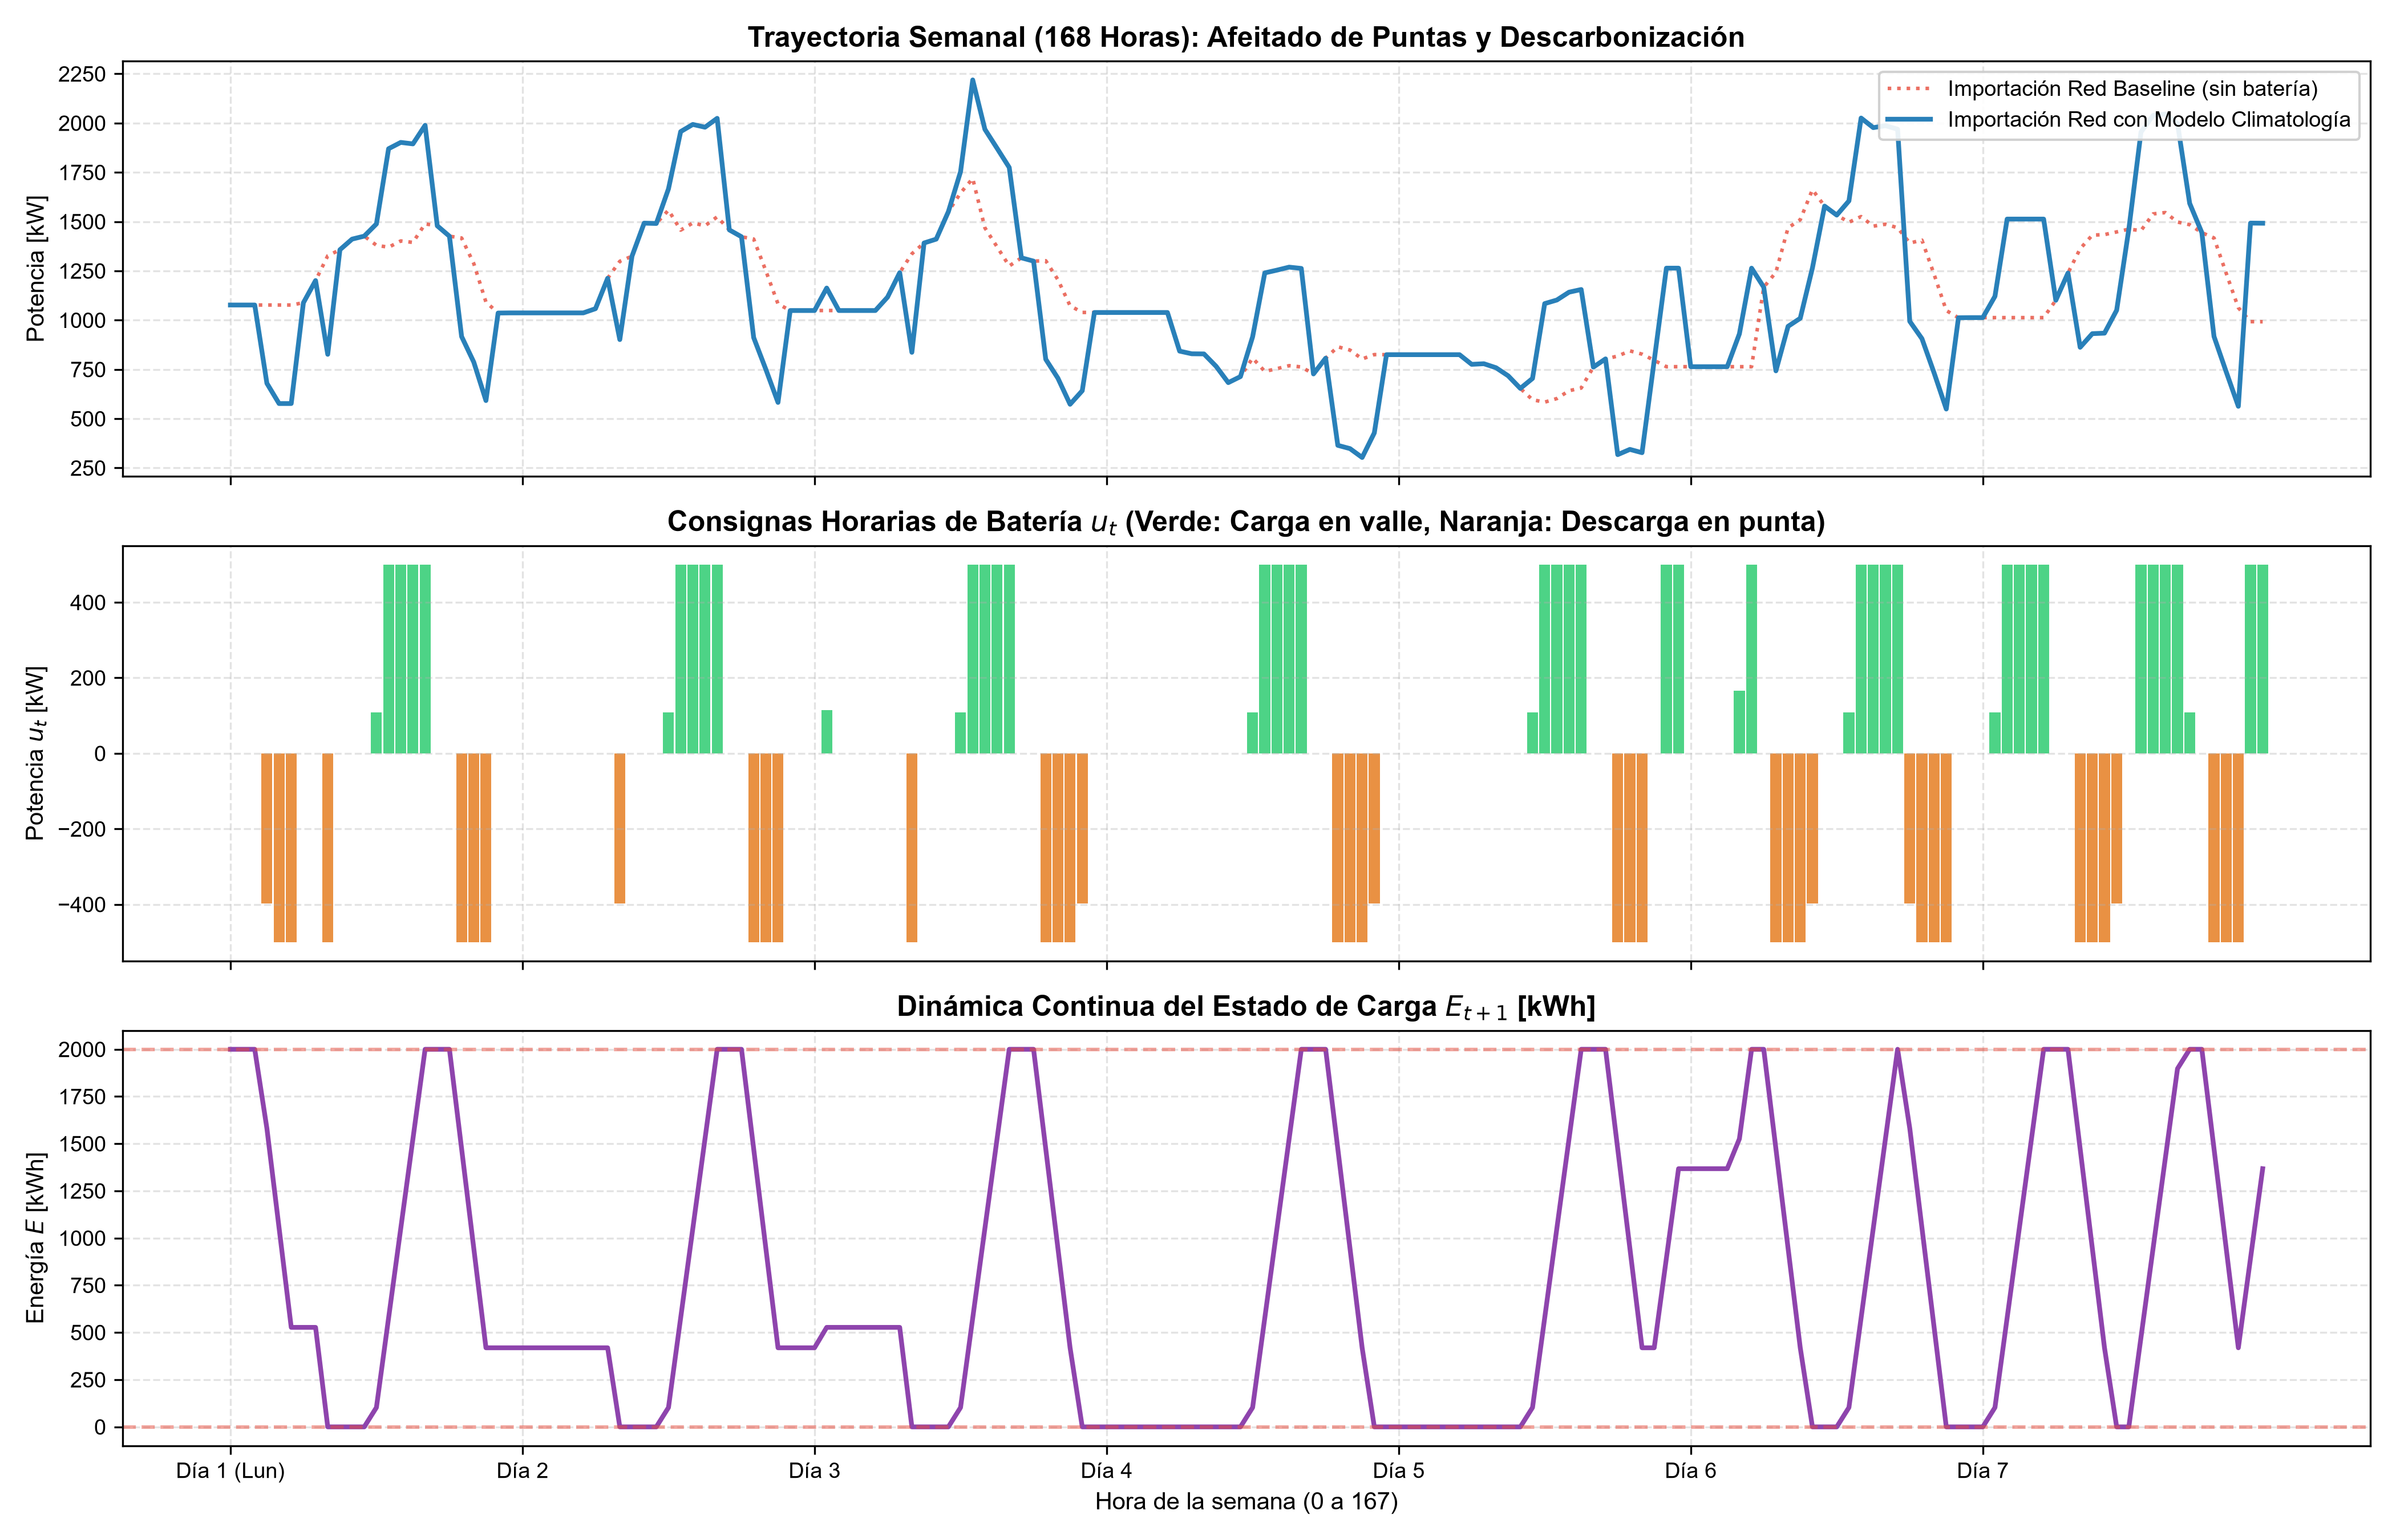
\includegraphics[width=0.92\linewidth]{fig/04_trayectoria_semana_completa.png}
\caption{Trayectoria semanal continua (168 horas). Afeitado continuo de picos de red y ciclos óptimos de batería sin saturación.}
\label{fig:semana}
\end{figure}

\section{Nivel 5: Validación Experimental y la Interfaz Animada}

\subsection{Protocolo Ciego de Validación (Pseudo-Test)}
Para garantizar la ausencia de filtración de datos (\emph{data leakage}), evaluamos los algoritmos sobre los días 15 a 21 de cada mes (12 semanas, 1.725 horas). Todos los parámetros del modelo se estimaron exclusivamente con los días de entrenamiento restantes.

\begin{table}[H]
\centering
\small
\begin{tabular}{lcccc}
\toprule
\textbf{Métrica de Evaluación} & \textbf{Línea Base (u=0)} & \textbf{Plantilla Oficial} & \textbf{Modelo Medias (Prueba 1)} & \textbf{Impacto Relativo} \\
\midrule
\textbf{Score Oficial (0--100)} & \textbf{0.00} & \textbf{0.00} & \textbf{\textcolor{verdeeco}{5.40}} & \textbf{+100\%} \\
Reducción CO$_2$ (\%) & 0.00\% & 0.98\% & \textbf{5.05\%} & +415\% \\
CO$_2$ Ahorrado Neto (kg) & 0.0 kg & 1.701.8 kg & \textbf{8.805.0 kg} & +7.103.2 kg \\
Reducción de Coste (\%) & 0.00\% & 2.20\% & \textbf{6.23\%} & +183\% \\
Coste Ahorrado Neto (\euro) & 0.00 \euro & 6.239.05 \euro & \textbf{17.670.51 \euro} & +11.431.46 \euro \\
Infracciones Físicas & 0 & 9 & \textbf{0 (Limpio)} & Sin penalización \\
Tiempo de Cómputo (s) & 0.94 s & 0.96 s & \textbf{10.06 s} & < 60 s \\
\bottomrule
\end{tabular}
\caption{Comparativa rigurosa en el conjunto de pseudo-test ciego (1.725 horas en 12 bloques).}
\end{table}

\begin{figure}[H]
\centering
\begin{minipage}{0.58\linewidth}
    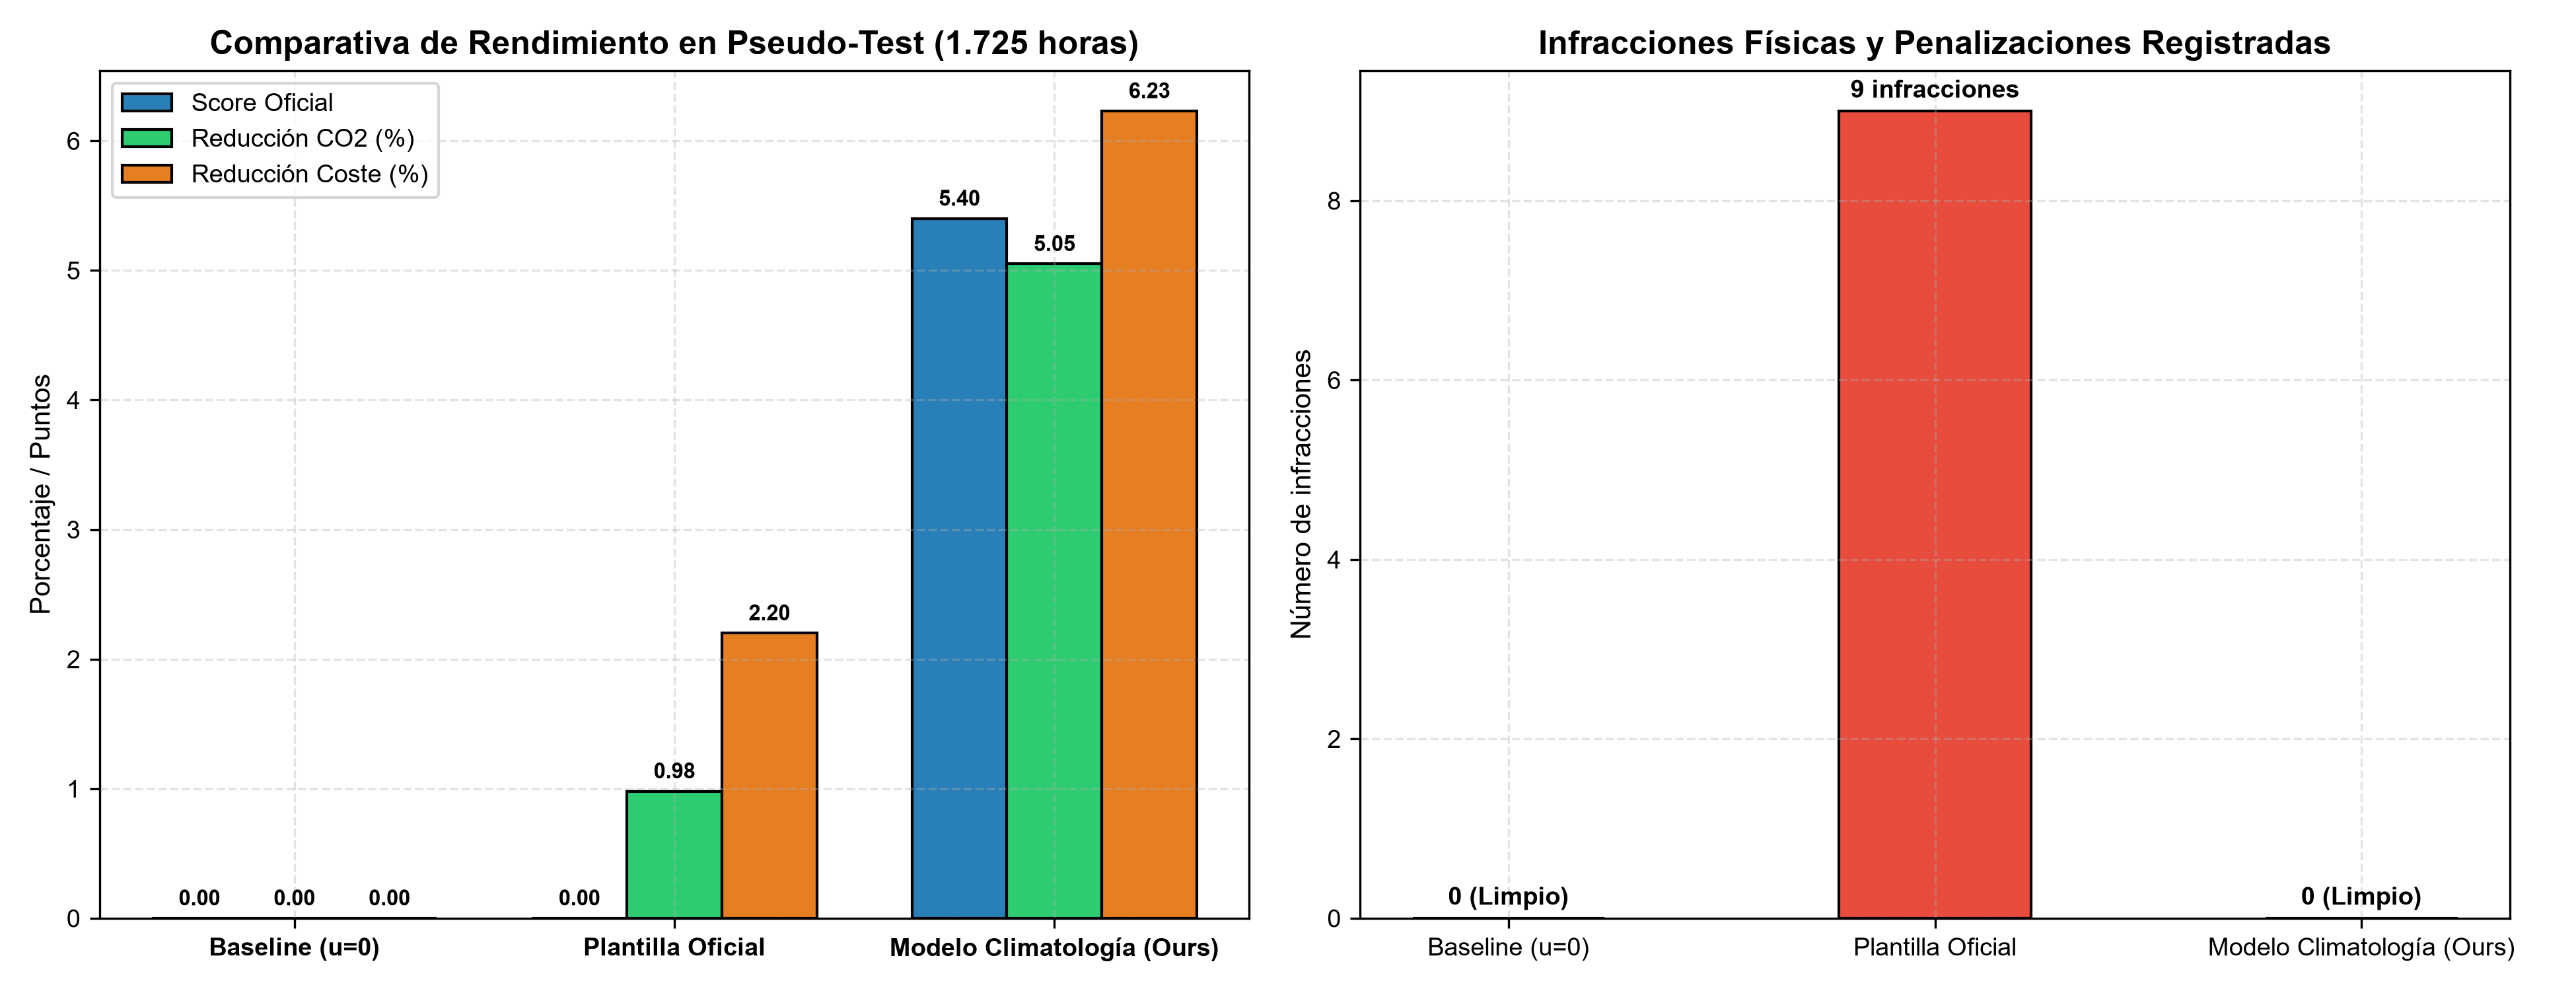
\includegraphics[width=\linewidth]{fig/05_comparativa_modelos.png}
    \caption{Comparativa de Score y ahorros.}
\end{minipage}\hfill
\begin{minipage}{0.38\linewidth}
    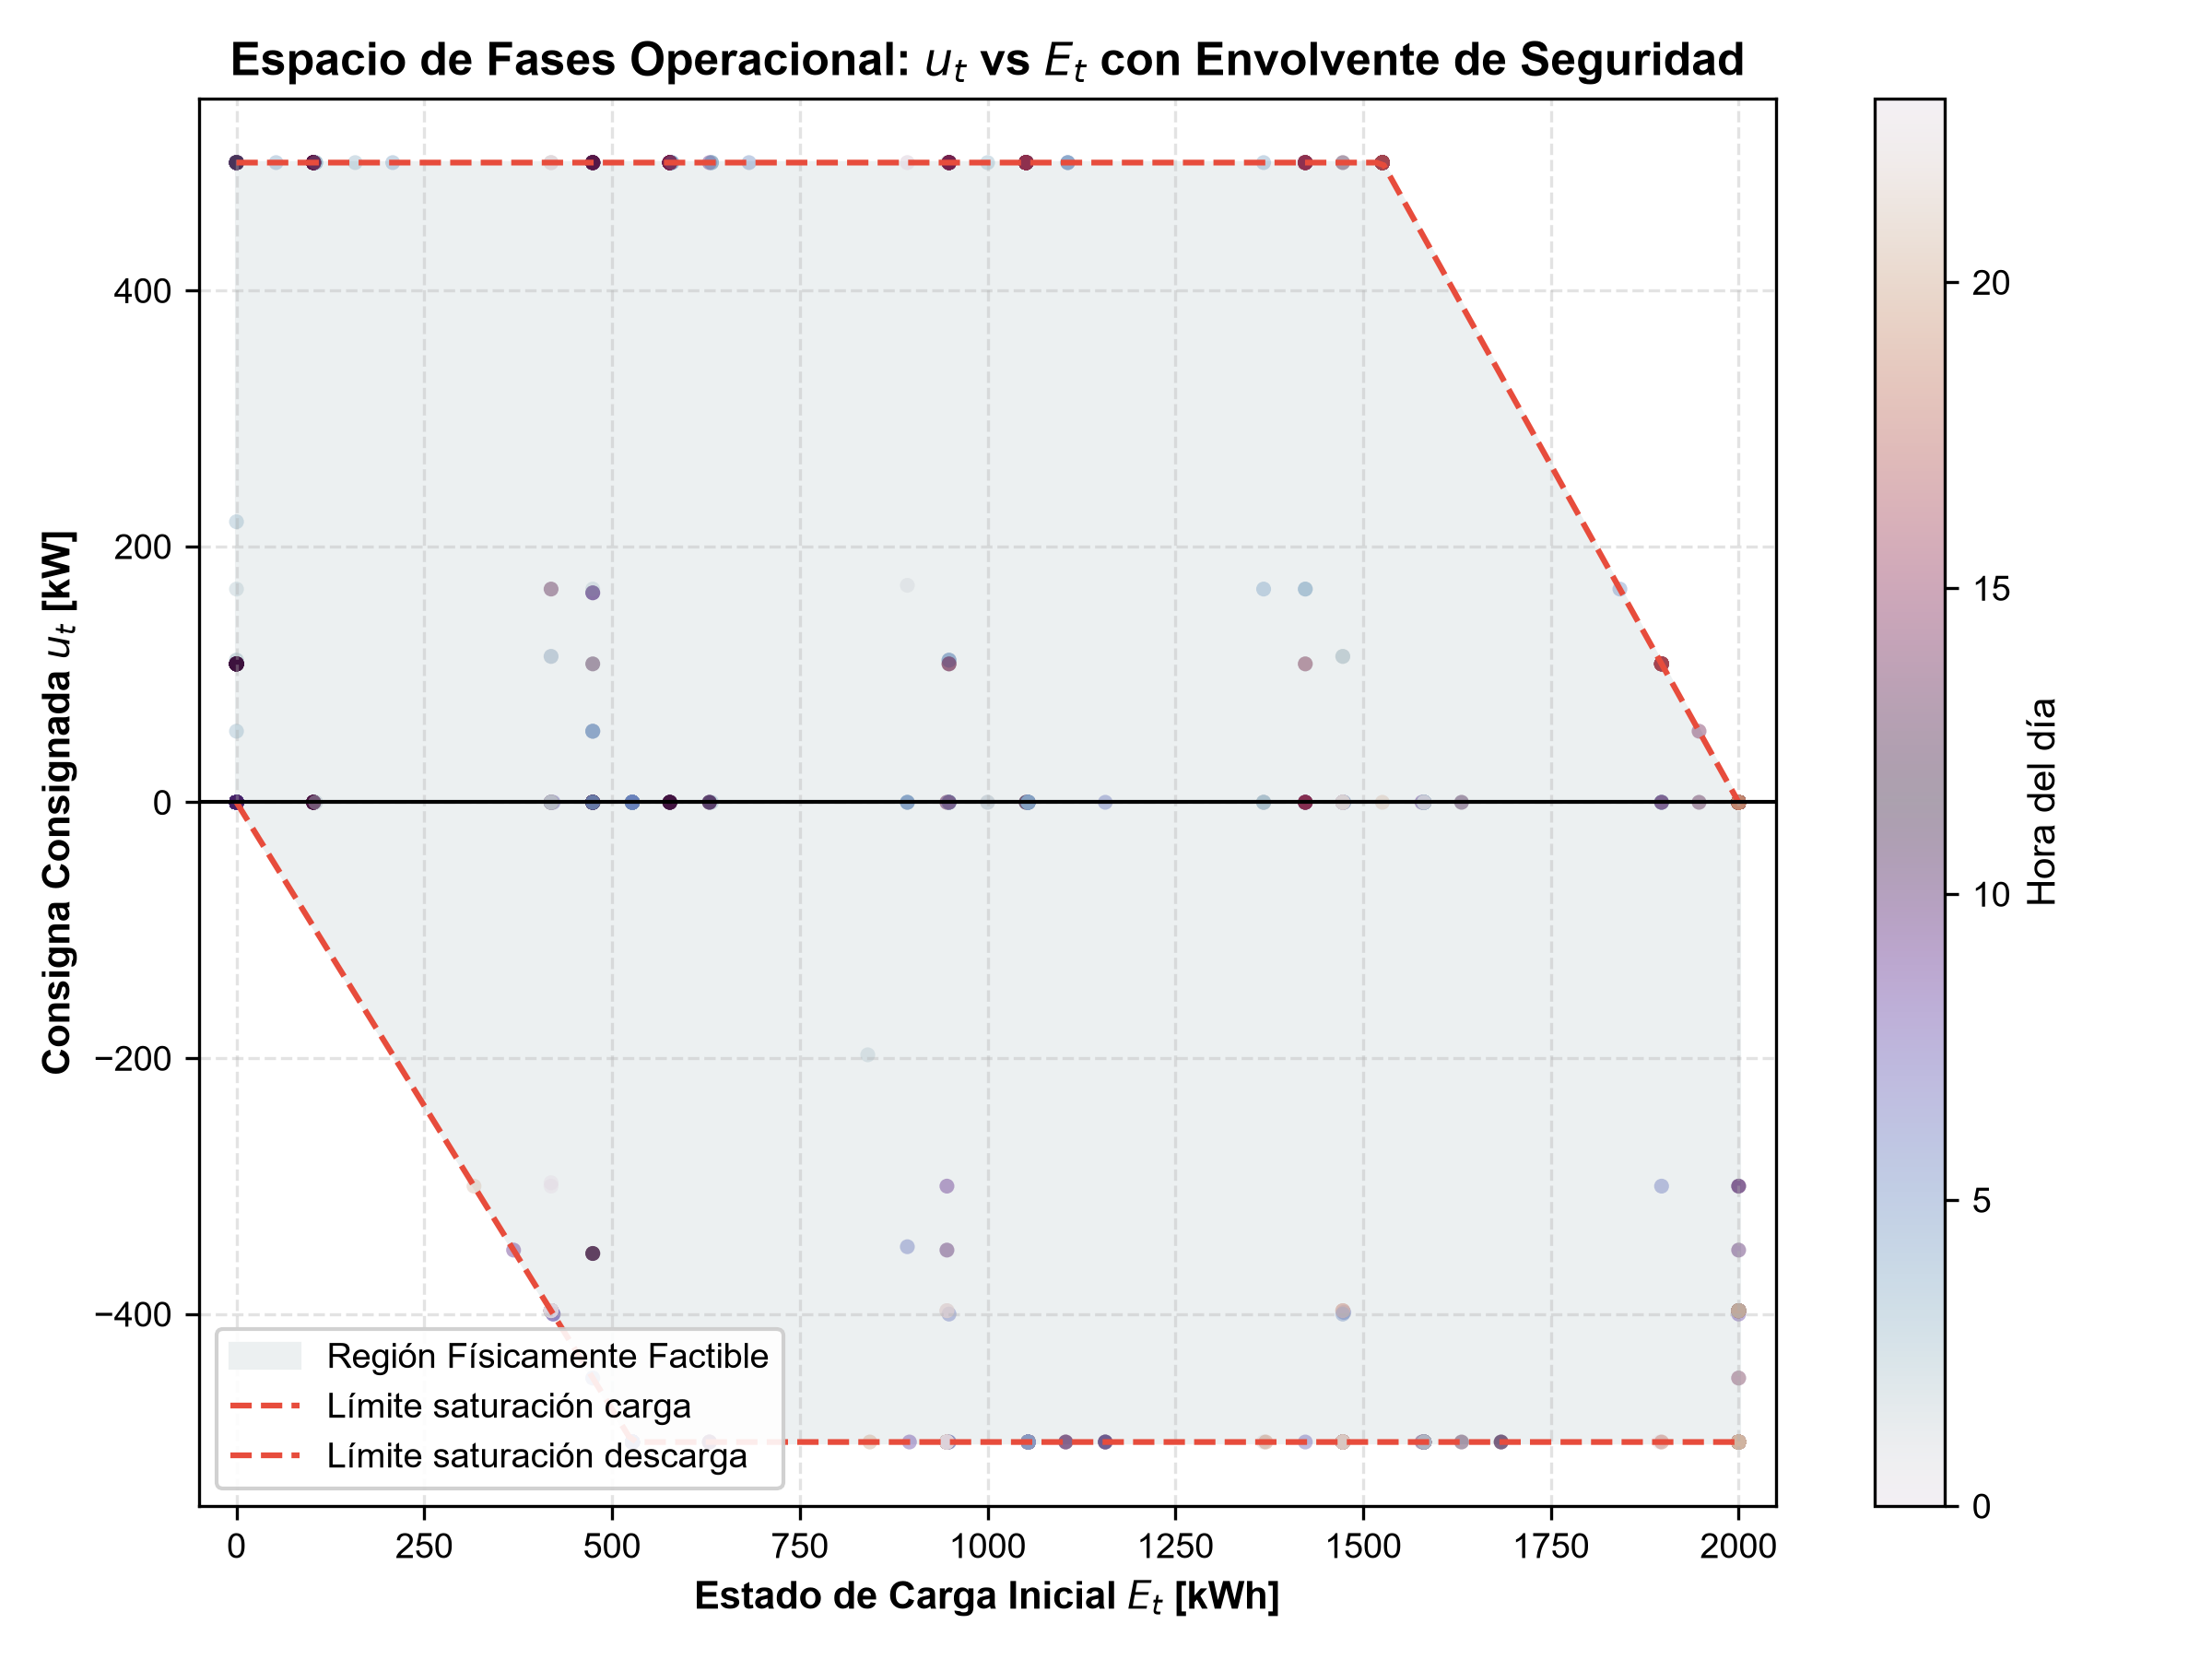
\includegraphics[width=\linewidth]{fig/06_dinamica_ut_vs_soc.png}
    \caption{Espacio operacional $u_t$ vs $E_t$.}
\end{minipage}
\end{figure}

\subsection{La Interfaz Web Animada e Interactiva}
Para visualizar cómo progresan las variables hora a hora y a lo largo de toda la semana, se desarrolló la aplicación interactiva autocontenida \texttt{interfaz\_animada.html}:
\begin{itemize}
    \item \textbf{Tanque Físico de Batería Animado:} Muestra el nivel exacto de energía $E_{t+1}$ en kWh (0 a 2.000 kWh) y porcentaje SOC con animación reactiva de fluido en tiempo real (verde brillante durante la carga y ámbar en descarga).
    \item \textbf{Tacómetro de Potencia $u_t$:} Indicador digital bidireccional entre $-500\text{ kW}$ y $+500\text{ kW}$.
    \item \textbf{Controles Temporales:} Reproducción automática con velocidad ajustable (0.5x a 10x), barra deslizadora horaria (0 a 167 h) y selector de día (Lunes a Domingo).
    \item \textbf{Gráfico Dinámico Sincronizado:} Traza las curvas de demanda, generación solar, importación con y sin batería, con una aguja vertical móvil que avanza a 60 fps en tiempo real.
\end{itemize}

\end{document}